\section{QFAST Algorithm}

\subsection{Top-Down vs Bottom-Up Synthesizers}
\begin{frame}
\frametitle{Top-Down vs Bottom-Up Synthesizers}
\begin{figure}
  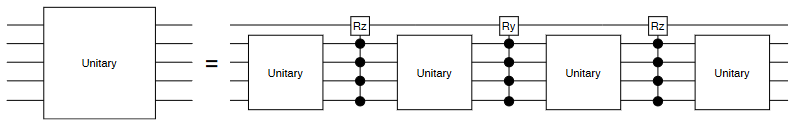
\includegraphics[width=\textwidth]{figure/top-down.png}
  \caption{Top-down synthesizers,decompose large unitaries into smaller ones while maintaining equality}
\end{figure}
% figure here
\end{frame}
\begin{frame}
  \frametitle{Top-Down vs Bottom-Up Synthesizers}
  \begin{figure}
    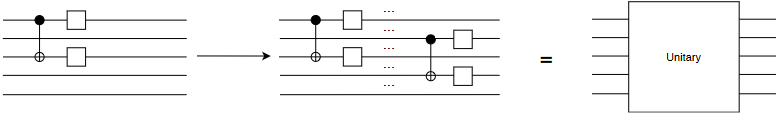
\includegraphics[width=\textwidth]{figure/bottom-up.png}
    \caption{Bottom-up synthesizers start with an empty circuit and build up to equality.}
  \end{figure}
  \begin{figure}
    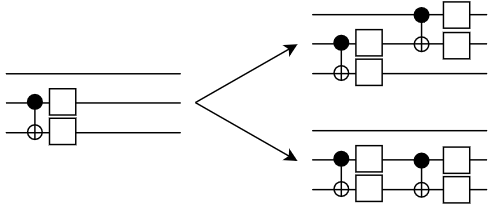
\includegraphics[width=.3\textwidth]{figure/Qsearch.png}
    \caption{QSearch uses native gates in synthesis and searches for structure in their circuit space.}
  \end{figure}
  % figure here
\end{frame}
\subsection{Introduction to QFAST Algorithm}
\begin{frame}
\frametitle{Basic idea to QFAST Algorithm}
\begin{itemize}
  \item use function to represent gates and circuits
  \item replaces expensive searches over circuit structures with numerical optimization
\end{itemize}
% work flow here
\end{frame}

\subsection{Gate Representation}
\begin{frame}
\frametitle{Gate Representation}

\begin{align}
  &F(Q, \vec{\alpha})=P_{Q}(G(\vec{\alpha}) \otimes I) P_{Q}^{T}\\
  &V(\vec{Q}, \vec{\alpha}, \vec{l})=\left(\sum_{Q \in \vec{Q}} l_{Q} \cdot P_{Q}\right)(G(\vec{\alpha}) \otimes I)\left(\sum_{Q \in \vec{Q}} l_{Q} \cdot P_{Q}^{T}\right)
\end{align}
where
\begin{align}
  G(\vec{\alpha})=e^{\mathrm{i}\left(\vec{\alpha} \cdot \sigma^{\vec{\otimes} n}\right)}
\end{align}
%  result formula
\end{frame}

\subsection{Cost Function for Optimization}
\begin{frame}
\frametitle{Cost Function for Optimization}
derive form Frobenius norm
\begin{align}
  \Delta\left(U_{C}, U_{T}\right)=1-\frac{\left|\operatorname{Tr}\left(U_{T}^{\dagger} U_{C}\right)\right|}{d}
\end{align}
% function here and how to optimize
\end{frame}
\begin{frame}
  \frametitle{work flow}
  \begin{itemize}
    \item decomposition
    \item instantiation
    \item recombination
  \end{itemize}
  \begin{figure}
    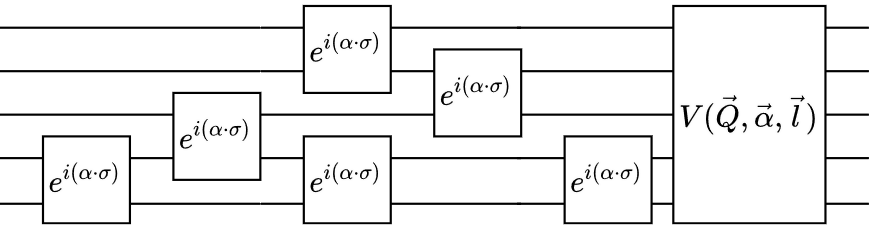
\includegraphics[width=.2\textwidth]{figure/decom.png}
  \end{figure}
\end{frame}

